%#Split: 02_purpose_plan  
%#PieceName: p02_purpose_plan
% p02_purpose_plan_00.tex
\KLBeginSubjectWithHeaderCommands{02}{}{研究目的・内容等}{2}{F}{}{\DCPDFirstSubjectPageStyle}{\DCPDDefaultPageStyle}

\section{研究目的・内容等}
%    <<最大 2ページ>>

%s02_purpose_plan_dcpd
%begin 研究目的と研究計画short留意事項なし ====================
%begin 研究計画における研究目的、研究方法、研究内容 ====================
\graysubsection{①研究計画における研究目的、研究方法、研究内容}
\vspace{20pt}
\sbsbsection{研究目的}

\setlength\intextsep{0pt}
\setlength\textfloatsep{0pt}
\begin{wrapfigure}{r}[0pt]{0.27\linewidth}
    \vspace{-2\baselineskip}
    \centering
    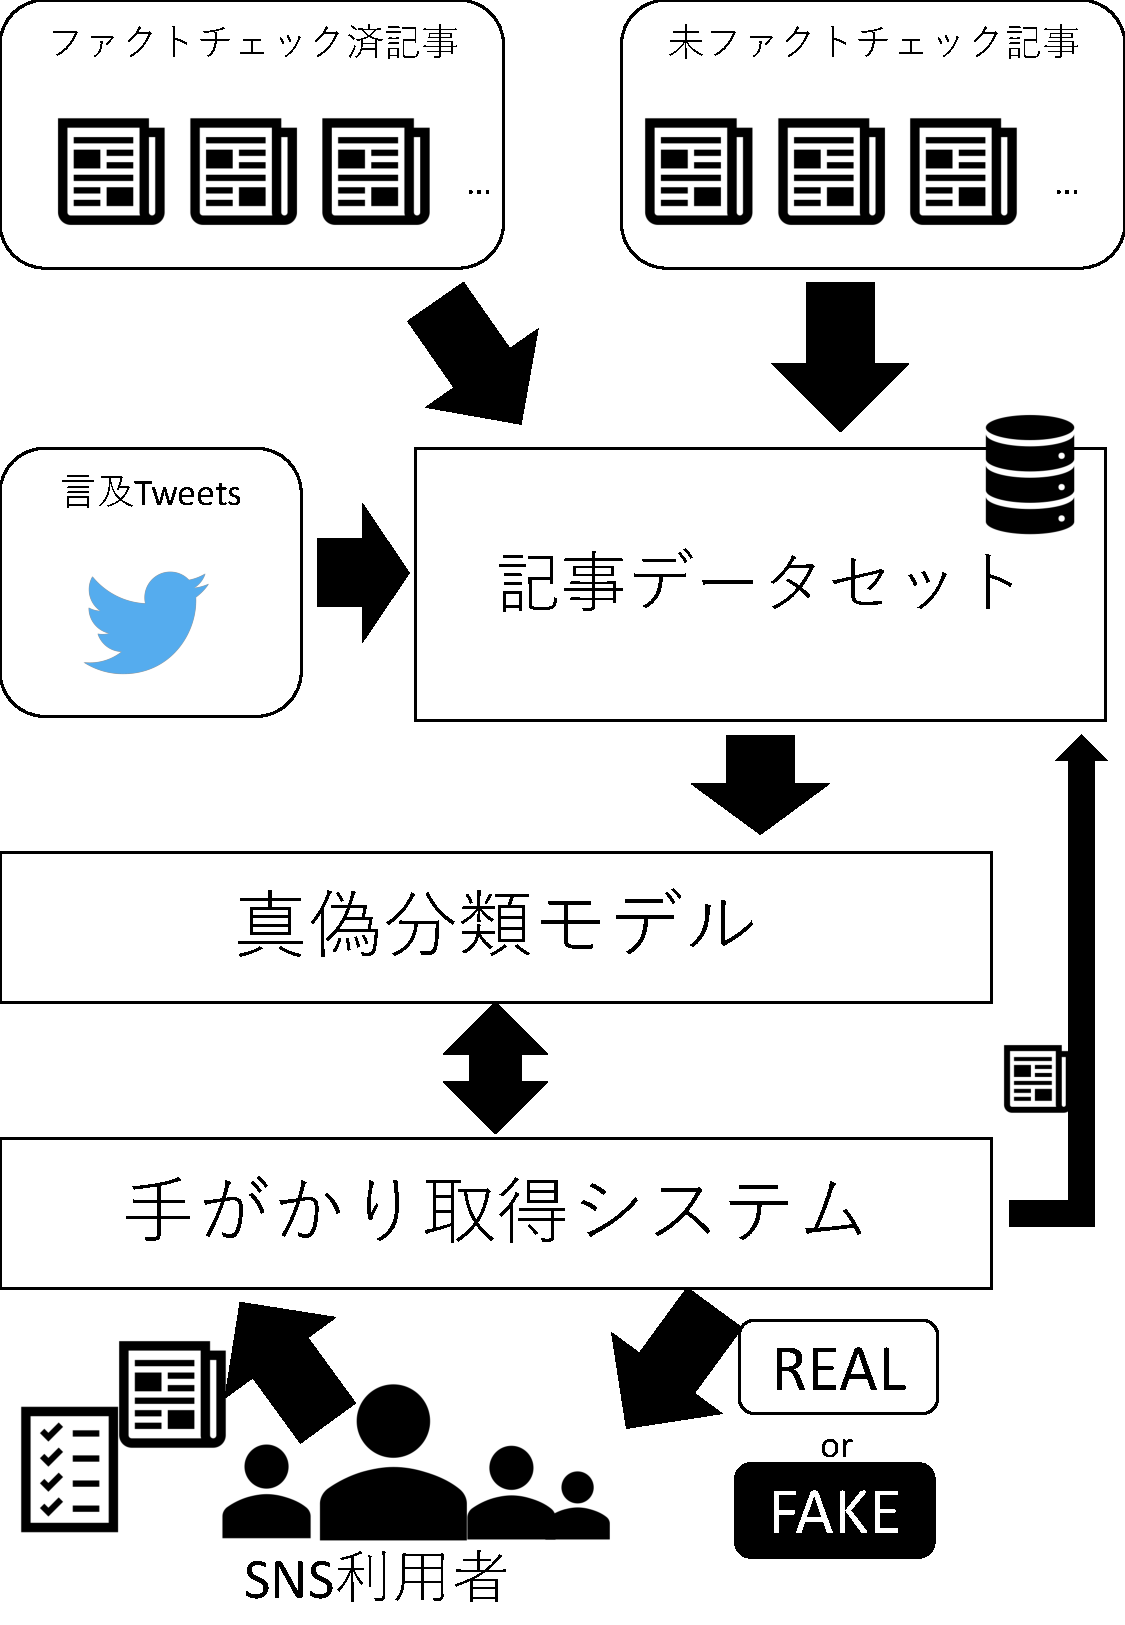
\includegraphics[width=0.27\textwidth]{figs/final.pdf}
    \vspace{-1.6cm} 
    \caption{真偽判断への手がかりを早期に取得する方法の例。}
    \label{fig:dataset}
    \vspace{-4\baselineskip}
\end{wrapfigure}

本研究では、利用者から検出に向けた手がかりを直接取得するシステムを構築する、新たなフェイクニュース早期検出の枠組みを作る。
またフェイクニュースの早期自動検出を日本語における実現・研究の促進を目指し、
データセットの作成から検出モデルの実装を目的とする。

\sbsbsection{研究方法・研究内容}

以下の3目標を目指し研究する。%本研究の最終形を図\ref{fig:dataset}に記す。
\vspace{-10pt}
\begin{description}
    \setlength{\parskip}{0cm}
    \setlength{\itemsep}{0cm}
    \item[目標Ⅰ] 早期検出に向け、SNS利用者から真偽判断の手がかりの提供を促す手がかり取得手法を検討する。
    \item[目標Ⅱ] 言語やトピックを問わず、普遍的な特徴から高精度な検出を行うフェイク検出モデルを開発する。
%    \item[目標Ⅲ] 実験に併せ日本語データセット作成に向け新たにファクトチェックされていない記事や、SNS上で記事に寄せられた既存のコメントや利用者情報等を収集する。
    \item[目標Ⅲ] 完成したシステムによるSNS利用者への拡散抑止力を主観評価実験により評価する。
    %\item[目標Ⅲ] 利用者に対して直接フェイクニュースの疑いを指摘すると同時にデータセットのアップデートを行うモデルを開発する。
\end{description}
\vspace{-10pt}
%end 研究計画における研究目的、研究方法、研究内容 ====================

%begin どのような計画で、何を、どこまで明らかにしようとするのか ====================
\graysubsection{②どのような計画で、何を、どこまで明らかにしようとするのか}
\vspace{20pt}
\sbsbsection{目標Ⅰ: 手がかり取得手法の検討(採用前 - 1年目)}
データセットとモデルの構築のみでは、今後のニュース内容の変化に対応することが難しい。
継続して社会の潮流の変化に対応するためには、データセットと検出方法及び利用者の反応を得る方法を工夫する必要がある。
%また、本研究の最終的な目標は国連のPause/ちょっと待って運動\cite{un}と同じくSNS利用者に対してフェイクニュース拡散前に利用者に再考を促して抑止を行うことである。
%この実現には、検出モデルの構築のみならず\underline{利用者に対し納得できる形で記事の疑わしさを提供するシステムの構築}により初めて実現する。
本研究では、SNS上で利用者から暗黙的に直接真偽判断への手がかりを得て早期検出の性能向上に繋げる新しいモデルを実装する。
実現形式として、
真偽判定に重要とみられる情報を引き出すためにキュレーターの役割であるリプライを送り、
\underline{利用者の真偽確認への調査活動を促進させて結果をリプライとして得る}形を想定している。
具体的には図\ref{fig:dataset}のようにまず記事とリプライ毎の重要度を既存研究\cite{shu2019kdd}で評価する。
次に重要とみられるリプライの前後関係から、
真偽判断の決定打となる重要リプライを引き出したリプライの傾向を得た上で、
その後新たな記事に対して重要リプライを得るためにリプライを生成し追加する。
%利用者に対し簡易的なチェックリスト(文体が感情的か・著者は明記されているか等)を課して回答を得たりする方法などを検討している。
このように真偽判断の決め手を得るために\underline{利用者へ能動的に働きかける形}を目指す。
%対象記事は英文とし、検出を行うモデルは既存手法を採用する予定である。
%本研究は、利用者がモデルに直接真偽を問い合わせるシステムを構築する。
%上記で実装したモデルに対して、利用者が記事内容を入力し問い合わせることで、
%真偽判断結果を提供すると共にデータセットへラベルなしニュースの追加を狙う。
%\underline{フェイクニュース拡散の抑止効果}を測定する。
%モデル提供が難しい場合は、データセットを公開し日本語におけるフェイクニュース早期検出研究促進を目指す。
%技術的チャレンジングさも書く
%利用者が疑わしい記事なのか早く知りたい→ファクトチェック結果を
%踏みとどまれの根拠をもたせる→国連
得られた成果は英語を対象としている点を加味し、採用1年目終了までに海外の自然言語処理を扱う学会への発表を予定している。

\sbsbsection{目標Ⅱ: 言語やトピックを問わず普遍的な特徴から検出するフェイク検出モデルの開発(1年目 - 2年目)}
\setlength\intextsep{0pt}
\setlength\textfloatsep{0pt}
\begin{wrapfigure}{r}[0pt]{0.7\linewidth}
    %\vspace{-2\baselineskip}
    \centering
    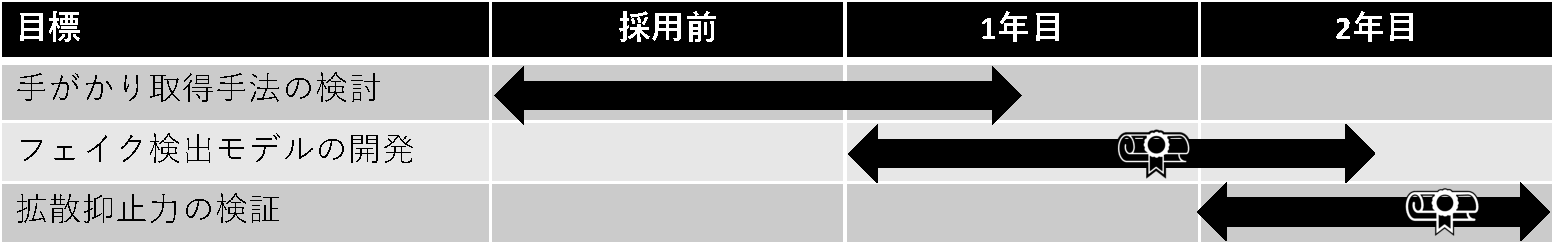
\includegraphics[width=0.7\textwidth]{figs/plan.pdf}
    \vspace{-1cm} 
    \caption{研究計画の年毎の流れと論文投稿予定時期。}
    \label{fig:plan}
    %\vspace{-3\baselineskip}
\end{wrapfigure}
教師あり学習の課題である高精度なラベル付けのコストを補うため、
不正確な弱いラベルを付けてから正確な分類を行う弱教師あり学習がある。
フェイクニュース検出においても、全コメントの賛否両論さやコメント投稿者の過去の投稿内容、そしてフォロー関係から弱いラベルを弱いラベル付けとして採用した方法がある\cite{shu2020leveraging}。
これら3種の弱いラベル付けも併せて学習することで、\underline{推論時は利用者の反応や手がかりを使わずに正確な早期検出}を実現した。
%日本語で実現を目指す場合、日本語での検出を行う研究が少なく言語の違いによる影響が未知数であるため\underline{大幅なモデルの改変を要する可能性}がある。
今回は別言語での早期検出実現に向けて3種の弱いラベル付けに加え、投稿者のプロフィールや使用された絵文字、ハッシュタグといったコメント情報で有用なものがないか模索する。
また開発の一環として日本語でのデータセットも作成するべく、ファクトチェック済のものを含む記事を収集する。
%日本語ファクトチェック結果の取得には、特定非営利活動法人ファクトチェック・イニシアティブが提供するFactCheck Naviを使用する。
%2021年4月現在で600超件のファクトチェック結果が公表されている。%おり、FIJが提供するガイドライン\cite{fij}に基づき9種類のレーティングが行われている。
%今回はその中で``誤り''、``虚偽''、``ミスリード''、``不正確''、``根拠不明''と評価された記事をフェイクと扱う。
%一方ファクトチェックにより正確と判断された事例はフェイクに比べて少な%く、2021年4月中旬現在FactCheck Naviの直近20件のファクトチェック結果は全てフェイクに該当する。
%いため、正確なニュースとして大手新聞社やロイター通信等の記事を収集する。
%また目標Ⅱに向けファクトチェックが行われておらず、正解ラベルがない記事も追加する。
%正確とみられるニュースは先述と同じく大手マスメディアが発信したニュースを扱い、
%疑わしい記事としてFactCheck Naviによって虚偽と複数回判断されたニュースサイトの他記事も収集対象とする。
%最終的には真偽合わせて\underline{ラベル付き記事を約1,200件}、\underline{ラベルなし記事を約5,000件以上}収集を目指す。
また利用者の反応として、全記事を対象にSNS上で寄せられたコメントとしてTwitterにて記事URLを含むツイートも収集する。
取得したデータセットは、可能な範囲で公開し日本語での研究の促進を目指す。

実験では、学習で記事と利用者の反応・手がかりを入力し、テストは記事のみを入力して早期検出時の状況を再現し既存の手法と比較する。
既知の手法と比較して学習・テストでデータセットを変更しても\underline{正確性が一般的に先行研究で良好とされる80\%以上}を維持していれば成功とみなす。
実現が難しいならば、要因がイベント由来なのか言語由来なのか追加で検証する。
本目標で得られた成果は採用2年目の半ばまでに、国内の言語処理学会を始めとした自然言語処理分野での発表を予定している。

%目標Ⅰの主観評価実験を並行する目標Ⅲの日本語での効果を測定する。

%\sbsbsection{目標Ⅲ: 日本語の記事・真偽を含むデータセットを作成する(1年目 - 2年目)}

%日本語での検出を実現するためには、まずはデータセットを作成する必要がある。
%データセット作成の全体の流れは図\ref{fig:dataset}の通りである。
%完全教師あり学習・弱教師あり学習に問わず最低限必要なものは記事情報とファクトチェック結果による真偽ラベルである。
%技術的チャレンジングさを強く主張する
%高速化させたい→そのために???を克服しなければならない
%学術的チャレンジングさ→日本語がない→言語的差異+研究がないので英語の流用でいいのか未知数

\sbsbsection{目標Ⅲ: SNS利用者への拡散抑止力の検証(2年目)}
目標Ⅰ・Ⅱによって完成された手がかり取得手法活用したフェイクニュース早期検出モデルが、実際にSNS利用者への拡散抑止力に繋がるか評価する。
実験ではSNS利用者を対象とした主観評価実験により、
\underline{利用者の共有判断への影響度を測定}する。
ここまで得られた成果は扱う分野の都合上、自然言語処理に加えてAIも対象に入れて採用期間終了までに国内外の学会や論文誌へ発表を想定している。

%end どのような計画で、何を、どこまで明らかにしようとするのか ====================

%begin 研究の特色・独創的な点 ====================
\graysubsection{③研究の特色・独創的な点}
\vspace{20pt}
\sbsbsection{本研究の特色}
\begin{itemize}
    \setlength{\parskip}{0cm}
    \setlength{\itemsep}{0cm}
    \item 能動的に\underline{利用者から情報提供を得て}フェイクニュースの検出と併せデータセットを拡大する点。
    \item \underline{日本語}を対象にフェイクニュースの自動検出を行う点。
    \item ファクトチェックの結果を待たず\underline{早期の検出}を目指す点。
\end{itemize}
\vspace{-17pt}
\sbsbsection{独創的な点: 先行研究との比較}
利用者の反応を利用する先行研究は、反応発生を待って取得する受動的な形であり、
形式もSNSプラットフォーム(Twitter, Instagram, Weibo, etc.)で差異がみられる。
一方自ら能動的に情報を収集する手法が申請書作成時は世界的に見られず、本研究計画が初となる。
本研究は\underline{能動的に利用者から手がかりを得る}枠組みを作り、今後\underline{主流SNSが変化しても早期検出の実現}を目指している。

また深層学習でフェイクニュースを自動検出する\underline{対象は英文に集中}し、
\underline{日本語はデータセットがなく}盛んではない。
言語に囚われず利用者による拡散された経緯で真偽を判断する研究もあるが\cite{tarek2020}、
依然として記事の内容を考慮した研究では日本語を対象としたものがない。
\vspace{-5pt}
\sbsbsection{独創的な点: 予想されるインパクト・将来の見通し}
総務省によるとSNS利用率は2019年で69\%を占める。
更にSNSマーケティング市場規模は2025年に1兆1,171億円まで成長する(出典:サイバー・バズ/デジタルインファクト調べ)。
% インシデントを重ねて書く
利用者の増加によって、今後フェイクニュースが\underline{謂れなき風評被害に悩む事例を増やし}、\underline{更に深刻な社会損害}の発生を懸念する。

本研究の完成で、これまで活発ではなかった日本語のフェイクニュースを早期検出するモデルの開発および提供が可能となる。
そのうえ本研究が目指す利用者から手がかりを得る方法は、SNSプラットフォームではなく利用者に依存する形であるため、\underline{SNS利用者からの情報提供がある限り持続可能な方法}である。
継続したSNS利用者への注意喚起や、ファクトチェックの担い手への補助システムへの活用
など様々な形式で、SNS上で騙される人を減らし\underline{社会的損害や風評被害を未然に防ぐ・軽減する}枠組み作りに貢献する。


%end 研究の特色・独創的な点 ====================

%begin 申請者が担当する部分 ====================
\graysubsection{④申請者が担当する部分}
本研究は所属研究室内でも萌芽的な取り組みで、環境・技術面の支援を除き\underline{申請者が中心部分を担当}する。
データセットの生成では、正確なニュースの取得へ大手マスメディアへ協力を求める可能性がある。
%end 申請者が担当する部分 ====================

%begin 受入研究機関と異なる研究機関での研究従事計画 ====================
\graysubsection{⑤受入研究機関と異なる研究機関での研究従事計画}
申請者は\underline{1年間タリン工科大学の言語技術研究所(Tanel Alumäe所長)で活動予定}である(p.8 成果\ref{enum:tobitate})。
当該分野は北米と欧州の研究が活発であることから、
強くフェイクニュース対策の重要性が叫ばれている地域の派遣先研究室で\underline{最前線の研究に従事}し、
COVID-19によって得ることが難しい状況である現状で国際的視点を得るために必要である。
%end 受入研究機関と異なる研究機関での研究従事計画 ====================

%\vspace{-3mm}
{\footnotesize 
\begin{twobibliography}{99}
    \setlength{\parskip}{0cm}
    \setlength{\itemsep}{0cm}
    \setcounter{enumiv}{9}
    %\bibitem{fij} FIJ. 2019: ファクトチェック・ガイドライン
    \bibitem{shu2019kdd} K. Shu, \textit{et al.} \textit{KDD '19}
    \bibitem{shu2020leveraging} K. Shu, \textit{et al.} \textit{ECML-PKDD 2020}
    %\bibitem{un} UNIC. \url{https://is.gd/UNIC_pause}. 2020
    \bibitem{tarek2020} T. Hamdi, \textit{et al.} \textit{ICDCIT 2020}
\end{twobibliography}
}
%end 研究目的と研究計画short留意事項なし ====================
% p02_purpose_plan_01.tex
\KLEndSubject{F}


